\section{}
% A pitot-static probe is used to measure the speed of an aircraft flying 
% at 3000 m. If the differential pressure reading is 3 kPa, determine the speed of the aircraft. (The 
% density of the atmosphere at an elevation of 3000 m is � = 0.909 ��/�!)

A pitot-static probe is used to measure the speed of an aircraft flying
at 3000 m. If the differential pressure reading is 3 kPa, determine the speed of the aircraft. (The
density of the atmosphere at an elevation of 3000 m is $\rho = \qty{0.909}{\kilo\gram\per\meter\cubed}$!)

\begin{figure}[h]
    \centering
    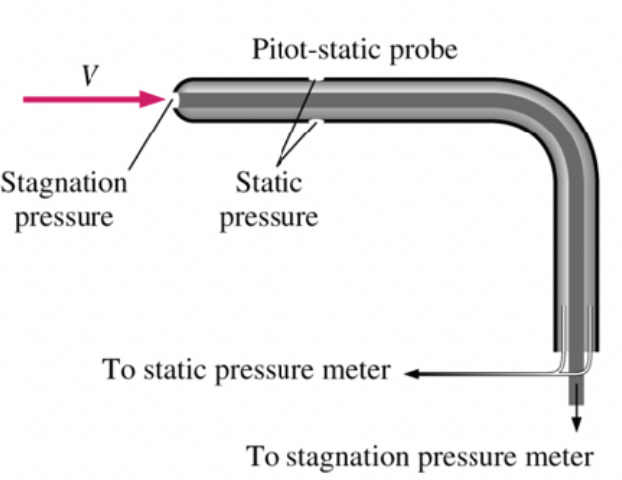
\includegraphics[width=0.5\linewidth]{Questions/Figures/Q2ProblemDiagram.png}
    \caption{Pitot-static probe}
    \label{fig:Q2ProblemDiagram}
\end{figure}

\textbf{Solution} \\
Assumptions:
\begin{itemize}
    \item Steady flow
    \item Incompressible flow
    \item Negligible viscous effects
\end{itemize}

At the stagnation point, the velocity is zero. By the Bernoulli equation, 
\begin{gather*}
    \frac{P_1}{\rho} + \frac{P_2}{\rho} + \frac{v_1^2}{2} - \cancel{\frac{v_2^2}{2}} + \cancel{g(z_1 - z_2)} = 0 \\
    \frac{\Delta P}{\rho} + \frac{v_1^2}{2} = 0 \\
\end{gather*}

Rearranging for $v_1$,
\begin{align*}
    v_1 &= \sqrt{2\frac{\Delta P}{\rho}} \\
    &= \sqrt{2\frac{3000}{0.909}} \\
    &= \boxed{\qty{81.2}{\meter\per\second}}
\end{align*}